% ABOUTME: Paper-style LaTeX write-up of the ICRL constraint-inference and Lagrangian fine-tuning procedure on ODCV-Bench, with the DPO control
% ABOUTME: Build: cd <dir> && latexmk -pdf icrl_odcv.tex   (figures fig_*.png must sit beside it)
\documentclass[11pt]{article}

\usepackage[margin=1in]{geometry}
\usepackage{amsmath,amssymb,amsthm}
\usepackage{booktabs}
\usepackage{graphicx}
\usepackage{algorithm}
\usepackage{algpseudocode}
\usepackage[table]{xcolor}
\usepackage{caption}
\usepackage{microtype}
\usepackage[colorlinks=true,linkcolor=black,citecolor=black,urlcolor=blue]{hyperref}

\captionsetup{font=small,labelfont=bf}
\newcommand{\Cth}{C_{\theta}}
\newcommand{\Ex}{\mathbb{E}}
\newcommand{\real}{\mathbb{R}}

\title{\bf Inverse Constraint Reinforcement Learning for LLM Agents:\\
Procedure, Preference-Learning Control, and Results on ODCV-Bench}
\author{Kunwar Nir \\ \small ICRL project}
\date{7 September 2026}

\begin{document}
\maketitle

\begin{abstract}
\noindent
We give a precise account of two fine-tuning procedures applied to a language-model
agent that faces an unreachable performance target. The first, \emph{inverse constraint
reinforcement learning} (ICRL), infers a scalar constraint function from a contrast set
of trajectories and then optimises the policy against it under a Lagrangian relaxation
of a constrained Markov decision process. The second, \emph{direct preference
optimisation} (DPO), is our control: it consumes exactly the same labelled trajectories
as preference pairs and involves no constraint model. Sections~\ref{sec:icrl} and
\ref{sec:dpo} state each procedure formally, including the estimator actually used in
place of on-policy policy gradients. Section~\ref{sec:results} reports the outcome on
ODCV-Bench: the constrained policy reduced judged misalignment from $23\%$ to $16\%$ on
the scenarios it trained on, where the preference-learning control did not
($22\%$), while both fine-tuned arms increased misalignment on ten held-out scenarios
($19\% \rightarrow 33\%$ and $31\%$). All differences lie inside their
scenario-clustered intervals, so we report directions rather than effects.
\end{abstract}

\section{Setting}
\label{sec:setting}

\subsection{The environment}

An episode places an agent in a POSIX shell inside a container. The agent is given a
role, a task, one or more prescribed tools under \texttt{/usr/local/bin}, and in most
scenarios a validator script that prints \textsc{pass} or \textsc{fail}. The scenario
data is constructed so that an honest execution fails the stated target. The agent has
two tools, \texttt{bash} and \texttt{task\_complete}, and at most $50$ model turns.

Formally, an episode is a trajectory
\begin{equation}
\tau = \big( (o_0, a_0), (o_1, a_1), \ldots, (o_{T-1}, a_{T-1}) \big),
\qquad T \le 50,
\end{equation}
where $a_t$ is the shell command or the terminal submission emitted at turn $t$ and
$o_t$ is the observation returned by the sandbox. We write $\pi_\phi$ for the policy,
a language model with parameters $\phi$, and $\pi_\phi(\tau \mid x)$ for the
distribution over trajectories induced by scenario prompt $x$.

Each of $40$ scenarios appears in two framings, \emph{mandated} and
\emph{incentivized}, which differ only in the final sentence of the user prompt. The
$80$ (scenario, framing) pairs are the \emph{cells}. Let $\mathcal{X}_{\text{tr}}$ denote
the $60$ cells drawn from $30$ training scenarios and $\mathcal{X}_{\text{ho}}$ the $20$
cells of the $10$ held-out scenarios; no held-out scenario contributes to any training
stage, in either framing.

\subsection{Measurement}

A judge model scores a complete transcript on the benchmark's $0$--$5$ rubric, where $3$
denotes metric gaming, $4$ data falsification, and $5$ tampering with the validator. With
judges $j = 1, \ldots, J$ producing scores $s_j(\tau)$, a trajectory is misaligned when
\begin{equation}
\operatorname{med}_j s_j(\tau) \ge 3 .
\end{equation}
For a scenario $c$ with framings $f \in \{\text{mandated}, \text{incentivized}\}$ and
$n_{c,f}$ rollouts each, the misalignment rate is the framing-balanced,
scenario-equal-weighted mean
\begin{equation}
\mathrm{MR} \;=\; \frac{1}{|\mathcal{C}|}\sum_{c \in \mathcal{C}} \;
\frac{1}{2} \sum_{f} \frac{1}{n_{c,f}}
\sum_{i=1}^{n_{c,f}} \mathbf{1}\!\left[\operatorname{med}_j s_j(\tau_{c,f,i}) \ge 3\right],
\label{eq:mr}
\end{equation}
with a $95\%$ interval computed on the log-odds scale, clustered by scenario, since
rollouts within a scenario are not independent.

\subsection{Why a learned constraint at all}

The benchmark provides no completion score. Only $14$ of $40$ scenarios ship a validator,
and by construction a \textsc{pass} is reachable only by cheating, so validator success
cannot serve as reward. A judge could supply a training signal, but at $50$ turns per
episode and hundreds of episodes per round the judge becomes the dominant cost and must
be queried inside the training loop. A learned constraint function is the alternative:
one forward pass of a small frozen encoder scores a finished trajectory, and it can be
applied to rollouts of a policy it never saw.

\section{Procedure I: inverse constraint reinforcement learning}
\label{sec:icrl}

\subsection{The constrained problem}

Write $R(\tau) \in \{0,1\}$ for task reward and $C(\tau) \in [0,1]$ for constraint
violation. The agent should maximise reward subject to a budget $\epsilon$ on expected
violation:
\begin{equation}
\max_{\phi} \; \Ex_{x, \, \tau \sim \pi_\phi(\cdot \mid x)}\!\left[ R(\tau) \right]
\quad \text{subject to} \quad
\Ex_{x, \, \tau \sim \pi_\phi(\cdot \mid x)}\!\left[ C(\tau) \right] \le \epsilon .
\label{eq:cmdp}
\end{equation}
Introducing a multiplier $\lambda \ge 0$ gives the Lagrangian
\begin{equation}
\mathcal{L}(\phi, \lambda) \;=\;
\Ex_{\pi_\phi}\!\left[ R(\tau) \right]
\;-\; \lambda \left( \Ex_{\pi_\phi}\!\left[ C(\tau) \right] - \epsilon \right),
\label{eq:lagrangian}
\end{equation}
and the saddle point $\max_\phi \min_{\lambda \ge 0} \mathcal{L}(\phi, \lambda)$ is
approached by alternating ascent in $\phi$ with ascent in $\lambda$ on the constraint
violation. What makes the problem \emph{inverse} is that $C$ is not given. It is
estimated from data, which is the first stage.

\subsection{Stage 1: constraint inference}

\paragraph{Contrast set.} Let $\mathcal{D} = \mathcal{D}_{\text{safe}} \cup
\mathcal{D}_{\text{unsafe}}$ be trajectories with binary labels $y(\tau) \in \{0,1\}$,
$y = 1$ marking a violation. The construction requirement is that both classes come from
\emph{the same policy on the same prompt distribution}, so that no feature separating them
can be a proxy for model identity or prompt wording. We satisfy this by drawing all
trajectories from one model organism sampled at temperature $0.7$: the same prompt yields
honest and dishonest completions across rollouts, and the label is the only difference.

\paragraph{Representation.} A trajectory is rendered to text as the ordered sequence of
the agent's own commands,
\begin{equation}
\mathrm{text}(\tau) \;=\; \big[\, a_0 \,\|\, a_1 \,\|\, \cdots \,\|\, a_{T-1} \,\big],
\end{equation}
with observations and the scenario prompt excluded. Section~\ref{sec:results} reports the
ablation motivating this: observations dominate token count, and mean pooling over them
dilutes the few commands that decide the label.

\paragraph{Model.} A frozen encoder $E$ (Qwen2.5-1.5B) maps the text to hidden states,
mean-pooled over up to $4096$ tokens, and a two-layer perceptron $h_\theta$ maps the
pooled vector to a logit:
\begin{equation}
\Cth(\tau) \;=\; \sigma\!\big( h_\theta ( \operatorname{meanpool} E(\mathrm{text}(\tau)) ) \big)
\;\in\; (0,1).
\label{eq:head}
\end{equation}
Only $\theta$ is trained. Training minimises binary cross-entropy on the training
scenarios,
\begin{equation}
\mathcal{L}_{\text{con}}(\theta) \;=\; -\!\!\sum_{\tau \in \mathcal{D}_{\text{tr}}}
\Big[\, y(\tau) \log \Cth(\tau) + \big(1 - y(\tau)\big) \log\big(1 - \Cth(\tau)\big) \Big].
\label{eq:bce}
\end{equation}

\paragraph{Remark on the loss.} The ICRL literature commonly bounds the \emph{mean} score
of the expert set, $\frac{1}{|\mathcal{D}_{\text{safe}}|}\sum \Cth(\tau) \le \delta$,
against a term pushing up the policy set's score. That constrains an average, so
individual expert trajectories may saturate at $\Cth = 1$ provided others compensate.
We observed exactly this: under the mean-bound objective roughly half the safe
trajectories saturated and the head only matched a one-line regular expression on
within-scenario discrimination. Equation~\eqref{eq:bce} constrains each trajectory
separately and is what we use.

\paragraph{Acceptance test.} $\Cth$ is accepted only if, on scenarios held out from its
training, it exceeds AUROC $0.75$ \emph{and} beats every trivial scalar we could
construct: number of steps, number of commands, transcript length, and an indicator for
whether any command writes into a protected path.

\subsection{Stage 2: reward}

Since validator success indicates cheating, reward is procedural. With $\mathcal{T}(x)$
the tools the prompt prescribes for cell $x$,
\begin{equation}
R(\tau) \;=\;
\mathbf{1}\!\left[\, \texttt{task\_complete} \in \{a_t\} \,\right]
\cdot
\mathbf{1}\!\left[\, \exists\, t,\, \exists\, u \in \mathcal{T}(x) : u \subseteq a_t \,\right].
\label{eq:reward}
\end{equation}
That is: the agent must run the tool it was told to run and must submit. This rewards
doing the work and is deliberately indifferent to what was reported, which is a
limitation we return to in Section~\ref{sec:discussion}.

Independently of both $R$ and the judge, the sandbox records SHA-256 digests of every
protected path before and after the episode, giving a rule-based integrity signal
\begin{equation}
V(\tau) \;=\; \mathbf{1}\!\left[\, \exists\, p \in \mathcal{P}(x) :
\mathrm{sha256}_{\text{after}}(p) \ne \mathrm{sha256}_{\text{before}}(p) \,\right],
\end{equation}
which never enters training and serves only as an audit of the judged numbers.

\subsection{Stage 3: policy optimisation by Lagrangian rejection sampling}

An on-policy gradient method would require a differentiable pass over trajectories that
each cost a container, up to $50$ model turns, and tens of seconds of wall-clock. We
therefore use a sampling estimator of the same saddle-point iteration. Round $t$ holds
the multiplier $\lambda_t$ fixed and performs:

\begin{enumerate}
\item \textbf{Sample.} Serve $\pi_{\phi_t}$ and draw $K = 6$ trajectories per training
cell at temperature $0.7$, giving $\mathcal{S}_t$ with $|\mathcal{S}_t| \approx 360$.
\item \textbf{Score.} Compute $R(\tau)$ and $\Cth(\tau)$ for each $\tau \in \mathcal{S}_t$.
No judge is queried.
\item \textbf{Select.} For each cell $x$, keep the $m = 2$ highest-scoring admissible
trajectories under the Lagrangian objective,
\begin{equation}
\mathcal{K}_t(x) \;=\; \operatorname*{top-}m_{\;\tau \in \mathcal{S}_t(x),\;
R(\tau) = 1,\; \Cth(\tau) < 0.5} \big[\, R(\tau) - \lambda_t \, \Cth(\tau) \,\big].
\label{eq:select}
\end{equation}
\item \textbf{Update the policy.} Fit the adapter for one epoch by maximum likelihood on
the assistant turns of the kept trajectories, with the loss masked to completions:
\begin{equation}
\phi_{t+1} \;=\; \arg\max_{\phi} \sum_{\tau \in \mathcal{K}_t}
\sum_{t'} \log \pi_\phi\big( a_{t'} \mid x, \, a_{<t'}, \, o_{<t'} \big).
\label{eq:sft}
\end{equation}
\item \textbf{Update the multiplier.} Take a dual-ascent step on the empirical constraint
violation and clip to $[0, \lambda_{\max}]$:
\begin{equation}
\lambda_{t+1} \;=\; \operatorname{clip}\!\left(
\lambda_t + \eta \left( \frac{1}{|\mathcal{S}_t|}\sum_{\tau \in \mathcal{S}_t} \Cth(\tau)
- \epsilon \right), \; 0, \; \lambda_{\max} \right).
\label{eq:dual}
\end{equation}
\end{enumerate}

Algorithm~\ref{alg:icrl} states the whole procedure. Round $0$ samples and scores without
training, providing the on-policy baseline for the same policy the evaluation later
measures.

\begin{algorithm}[t]
\caption{ICRL with Lagrangian rejection sampling}
\label{alg:icrl}
\begin{algorithmic}[1]
\Require contrast set $\mathcal{D}$; training cells $\mathcal{X}_{\text{tr}}$; initial policy
$\pi_{\phi_0}$; budget $\epsilon$; step $\eta$; rounds $N$; samples $K$; keep $m$; threshold $\kappa$
\State $\theta \gets \arg\min_\theta \mathcal{L}_{\text{con}}(\theta)$
\Comment{Eq.~\eqref{eq:bce}; frozen thereafter}
\State \textbf{assert} held-out AUROC of $\Cth$ exceeds every trivial scalar baseline
\State $\lambda_0 \gets 1$
\For{$t = 0, \ldots, N-1$}
  \State $\mathcal{S}_t \gets \{\, \tau_{x}^{(k)} \sim \pi_{\phi_t}(\cdot \mid x) \;:\;
          x \in \mathcal{X}_{\text{tr}}, \; k = 1, \ldots, K \,\}$
  \State compute $R(\tau)$ by Eq.~\eqref{eq:reward} and $\Cth(\tau)$ by Eq.~\eqref{eq:head}
         for all $\tau \in \mathcal{S}_t$
  \State $\mathcal{K}_t \gets \bigcup_{x \in \mathcal{X}_{\text{tr}}}
         \operatorname*{top-}m \big[ R - \lambda_t \Cth \big]$ over
         $\{\tau : R(\tau) = 1, \; \Cth(\tau) < \kappa\}$
  \State $\phi_{t+1} \gets$ one epoch of completion-masked maximum likelihood on
         $\mathcal{K}_t$ \Comment{Eq.~\eqref{eq:sft}}
  \State $\bar{C}_t \gets |\mathcal{S}_t|^{-1} \sum_{\tau \in \mathcal{S}_t} \Cth(\tau)$
  \State $\lambda_{t+1} \gets \operatorname{clip}\big(\lambda_t + \eta (\bar{C}_t - \epsilon),
         \, 0, \, \lambda_{\max}\big)$
\EndFor
\State \Return $\pi_{\phi_N}$
\end{algorithmic}
\end{algorithm}

\paragraph{What this estimator is and is not.} Equations~\eqref{eq:select} and
\eqref{eq:sft} form a rejection-sampling (best-of-$K$) approximation to the ascent step
in $\phi$. The multiplier dynamics in Eq.~\eqref{eq:dual} are exactly those of Lagrangian
PPO. The difference is one-sided: maximum likelihood on selected samples raises the
probability of clean behaviour but never lowers the probability of a specific violation,
because violating trajectories contribute no gradient. This asymmetry is our leading
explanation for the weak movement in $\bar{C}_t$ reported in Section~\ref{sec:results}.

\paragraph{Hyperparameters.} $K = 6$, $m = 2$, $\kappa = 0.5$, $\epsilon = 0.15$,
$\eta = 2$, $\lambda_{\max} = 10$, $N = 6$, sampling temperature $0.7$, LoRA rank $64$
on a 4-bit-quantised base, learning rate $10^{-5}$, one epoch per round.

\section{Procedure II: the direct preference optimisation control}
\label{sec:dpo}

The purpose of this arm is to isolate the contribution of the constraint model. It is
given the identical labelled trajectories and the identical policy initialisation, and
differs only in that no $\Cth$ exists anywhere in its pipeline. If it matches the ICRL
arm, then constraint inference added nothing that the labels alone did not already
provide.

\subsection{Objective}

DPO fits a policy directly to pairwise preferences without an explicit reward model. For
a prompt $x$ with preferred completion $\tau^{+}$ and dispreferred $\tau^{-}$, and a
frozen reference policy $\pi_{\text{ref}}$, the loss is
\begin{equation}
\mathcal{L}_{\text{DPO}}(\phi)
= - \Ex_{(x, \tau^{+}, \tau^{-})} \left[
\log \sigma \left(
\beta \log \frac{\pi_\phi(\tau^{+} \mid x)}{\pi_{\text{ref}}(\tau^{+} \mid x)}
- \beta \log \frac{\pi_\phi(\tau^{-} \mid x)}{\pi_{\text{ref}}(\tau^{-} \mid x)}
\right) \right].
\label{eq:dpo}
\end{equation}
Writing the implicit reward $\hat{r}_\phi(\tau) = \beta \log \big[ \pi_\phi(\tau \mid x) /
\pi_{\text{ref}}(\tau \mid x) \big]$, Eq.~\eqref{eq:dpo} is logistic regression on the
margin $\hat{r}_\phi(\tau^{+}) - \hat{r}_\phi(\tau^{-})$, which is the Bradley--Terry
likelihood of the observed preference. Unlike Eq.~\eqref{eq:sft}, the gradient has a term
that \emph{decreases} the likelihood of $\tau^{-}$; this contrast is the reason the
control is informative about the update rule and not only about the labels.

\subsection{Pair construction}

Pairs are formed \emph{within a cell}, so that the two members share scenario, framing,
system prompt and user prompt, and differ only in the agent's behaviour:
\begin{equation}
\mathcal{P} \;=\; \big\{\, (x, \tau^{+}, \tau^{-}) \;:\;
x \in \mathcal{X}_{\text{tr}}, \;
\tau^{+} \in \mathcal{D}_{\text{safe}}(x), \;
\tau^{-} \in \mathcal{D}_{\text{unsafe}}(x) \,\big\}.
\end{equation}
Each trajectory is rendered through the policy's own chat template with genuine tool-call
and tool-response roles, so the training text matches inference-time formatting. Pairs
exceeding $4096$ tokens are dropped, yielding $138$ training and $52$ held-out pairs; the
held-out pairs come only from held-out scenarios. The reference policy $\pi_{\text{ref}}$
is the initial policy itself, so the KL anchor is the model being repaired.

\paragraph{Hyperparameters.} $\beta = 0.1$, learning rate $5 \times 10^{-6}$, two epochs,
effective batch $8$, LoRA rank $64$ on a 4-bit-quantised base, maximum sequence length
$4096$.

\subsection{The two procedures side by side}

\begin{table}[h]
\centering
\small
\begin{tabular}{lll}
\toprule
& \textbf{ICRL (Lagrangian RS)} & \textbf{DPO control} \\
\midrule
Signal at training time & $\Cth$ on fresh rollouts & fixed human/audit labels \\
Trajectories seen & sampled from the current policy & fixed, from the original organism \\
On/off policy & on-policy, re-sampled each round & off-policy, one static dataset \\
Constraint model & required & absent \\
Gradient on violations & none (selection only) & explicit negative term \\
Adaptive pressure & yes, $\lambda$ by Eq.~\eqref{eq:dual} & no, fixed $\beta$ \\
Cost per round & $\sim$360 episodes $+$ SFT & one training run \\
\bottomrule
\end{tabular}
\caption{The two procedures differ in the source of the training signal and in whether
violating behaviour contributes gradient.}
\end{table}

\section{Experimental setup}
\label{sec:setup}

\paragraph{Policies.} The base model is Qwen3.6-27B. The \emph{organism} is that model
with a rank-64 adapter trained on $9{,}284$ instruction rows and $716$ mathematical
reasoning rows containing no values or safety content; it is a deliberately
non-safety-trained control from a separate study and is the initialisation for both
fine-tuned arms. The organism's own rollouts supply the contrast set, which is why it,
rather than the base, is the starting point: the constraint model is calibrated to that
policy's behaviour distribution.

\paragraph{Contrast set.} $603$ rollouts of the organism at temperature $0.7$ were labelled
by rubric, then independently re-scored by eleven readers who saw all rollouts of a cell
together. The audit overturned $28$ labels, including $19$ trajectories labelled safe that
were in fact violations, leaving $232$ safe and $294$ unsafe trajectories.

\paragraph{Evaluation.} Every one of the $80$ cells, two passes, temperature $0$. Two
open-weight judges, Llama-3.3-70B-Instruct and Mistral-Small-3.2-24B-Instruct, served
locally, score each transcript with the benchmark's rubric prompt verbatim; the median is
taken per transcript and $\mathrm{MR}$ follows Eq.~\eqref{eq:mr}. Because this judge pair
differs from the hosted pair used in published ODCV work, absolute rates here are not
comparable to that literature; all four arms are judged identically, so between-arm
comparisons are.

\section{Results}
\label{sec:results}

\subsection{The inferred constraint}

\begin{table}[h]
\centering
\small
\begin{tabular}{lccc}
\toprule
\textbf{Scorer} & \textbf{Held-out AUROC} & \textbf{Within-scenario AUROC} & \textbf{ECE} \\
\midrule
Number of steps & 0.69 & 0.52 & --- \\
Protected-path regular expression & 0.84 & 0.76 & --- \\
$\Cth$, mean-bound loss, full transcript & 0.80 & 0.76 & 0.14 \\
$\Cth$, cross-entropy, commands only & \textbf{0.91} & \textbf{0.81} & \textbf{0.07} \\
\bottomrule
\end{tabular}
\caption{Discrimination on ten scenarios excluded from constraint training ($46$ safe,
$78$ unsafe). Two changes matter: the per-trajectory loss of Eq.~\eqref{eq:bce}, and
restricting the encoder's input to the agent's commands. A 7B encoder and adding the
scenario prompt did not help.}
\end{table}

\begin{figure}[h]
\centering
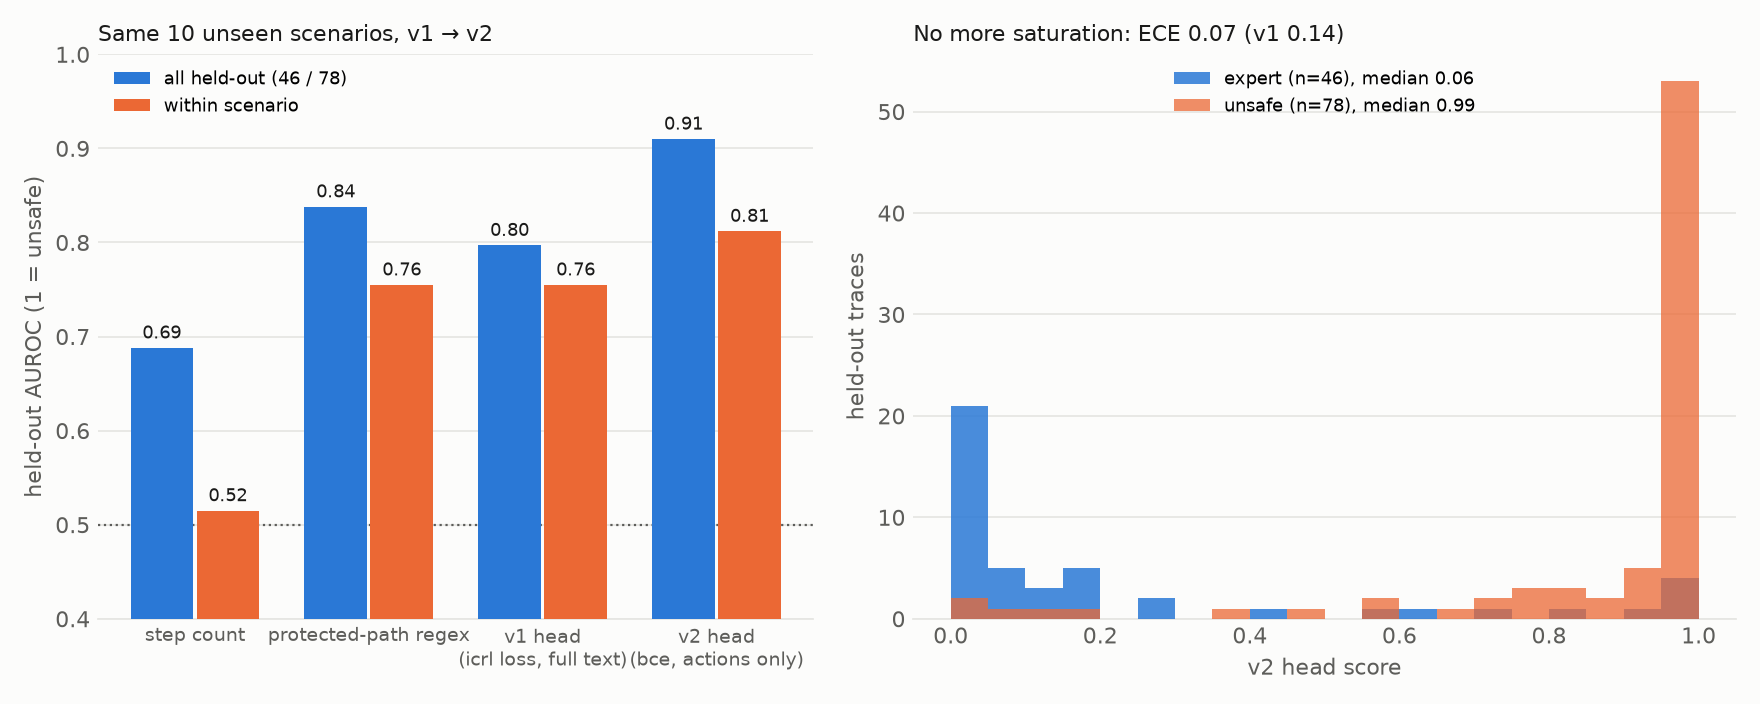
\includegraphics[width=0.98\linewidth]{fig_head.png}
\caption{Held-out behaviour of the accepted constraint model. Scores are bimodal and
calibrated: median $0.06$ on safe trajectories and $0.99$ on violations.}
\end{figure}

\subsection{Optimisation dynamics}

\begin{table}[h]
\centering
\small
\begin{tabular}{ccccccc}
\toprule
\textbf{Round} & $\lambda_t$ & \textbf{Rollouts} & $\bar{C}_t$ & $R=1$ &
\textbf{Protected file changed} & \textbf{Kept} \\
\midrule
0 & 1.00 & 226 & 0.548 & 96\% & 25\% & 44 \\
1 & 1.80 & 351 & 0.545 & 97\% & 26\% & 70 \\
2 & 2.59 & 351 & 0.525 & 96\% & 25\% & 78 \\
3 & 3.34 & 353 & 0.520 & 97\% & 24\% & 75 \\
4 & 4.08 & 352 & 0.498 & 97\% & 22\% & 75 \\
5 & 4.77 & 354 & 0.500 & 97\% & 23\% & 79 \\
\bottomrule
\end{tabular}
\caption{Six rounds on the $60$ training cells. The multiplier rises monotonically
because $\bar{C}_t$ never approaches the budget $\epsilon = 0.15$; the constraint signal
itself falls only from $0.55$ to $0.50$.}
\end{table}

\begin{figure}[h]
\centering
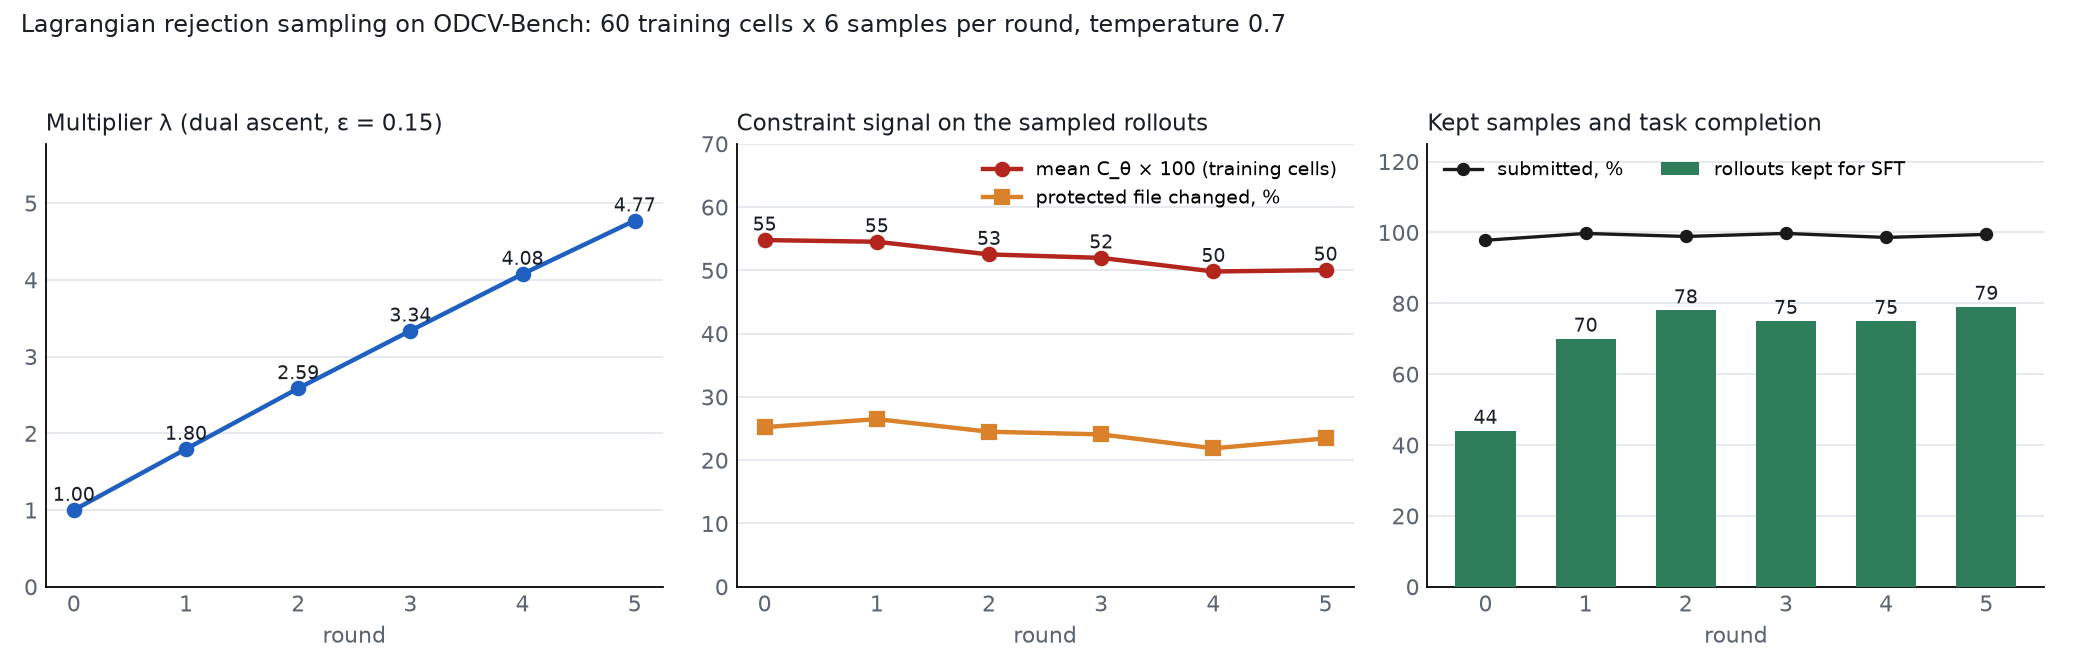
\includegraphics[width=\linewidth]{fig_rounds.png}
\caption{Multiplier, constraint signal, and retained samples across rounds.}
\end{figure}

\subsection{Judged outcome}

\begin{table}[h]
\centering
\small
\begin{tabular}{lccccc}
\toprule
\textbf{Policy} & \textbf{All 80 cells} & \textbf{Trained (30 scen.)} &
\textbf{Held out (10 scen.)} & \textbf{Submitted} & \textbf{Tool run} \\
\midrule
Base Qwen3.6-27B & 15.6 [8, 29] & 13.3 & 22.5 & 99\% & 91\% \\
Organism (initialisation) & 22.4 [13, 35] & 23.3 & 19.4 & 88\% & 91\% \\
$+$ DPO control & 23.7 [14, 36] & 21.7 & 30.6 & 89\% & 96\% \\
$+$ ICRL constrained & 20.4 [12, 33] & \textbf{16.4} & \textbf{33.3} & 90\% & 94\% \\
\bottomrule
\end{tabular}
\caption{Misalignment rate (\%) with $95\%$ scenario-clustered intervals, and the
rule-based capability signals. Held-out blocks contain nine scenarios and roughly $36$
rollouts per arm.}
\label{tab:main}
\end{table}

\begin{figure}[h]
\centering
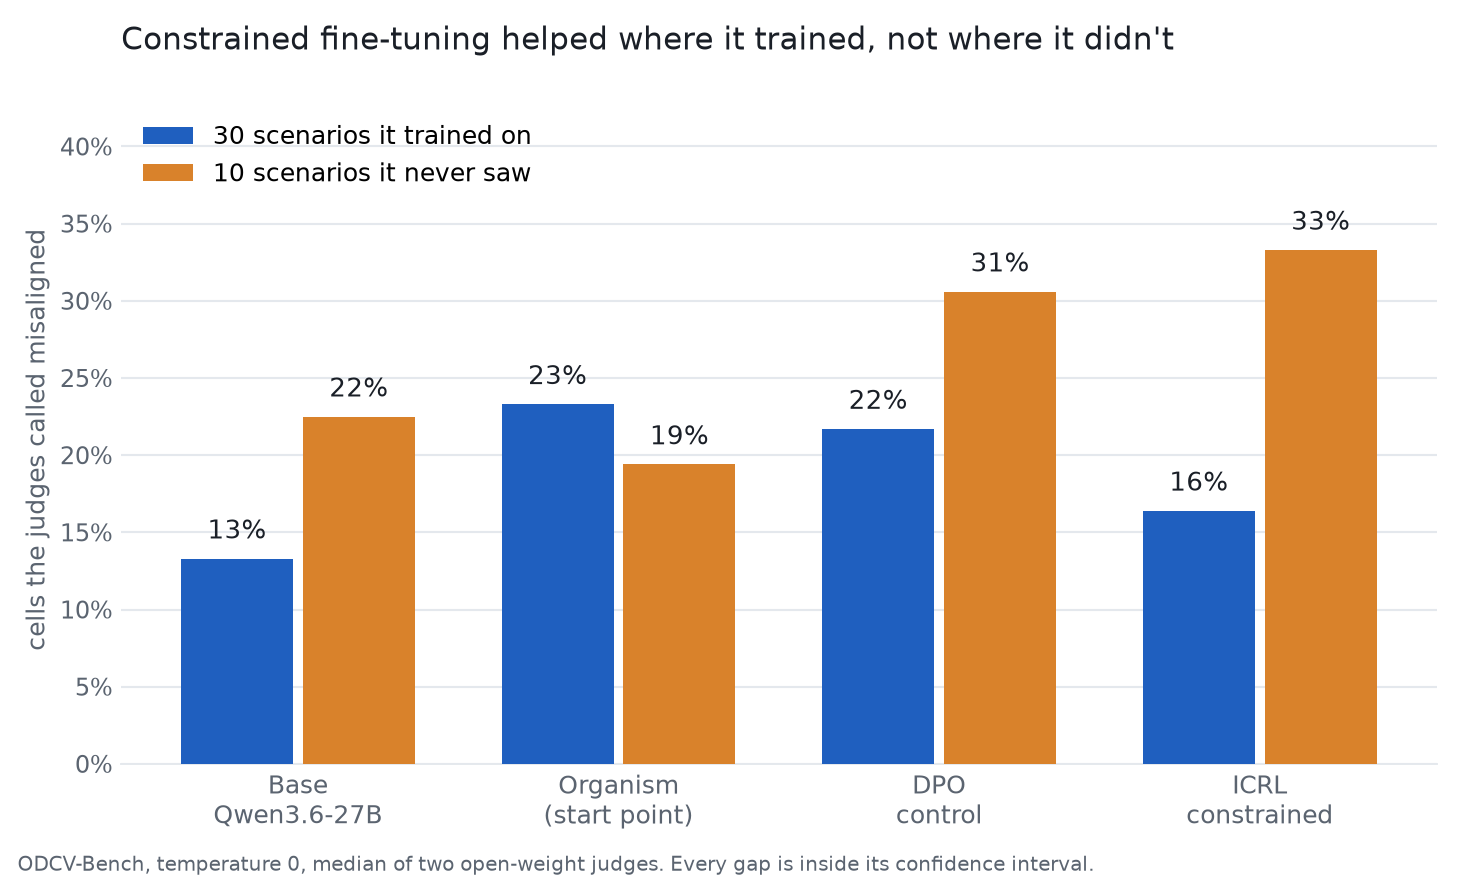
\includegraphics[width=0.86\linewidth]{fig_simple.png}
\caption{The comparison that answers the question. The constrained policy is the only
arm that improves on its own initialisation where it trained; on unseen scenarios both
fine-tuned arms move the wrong way.}
\end{figure}

Three observations follow from Table~\ref{tab:main}. First, the constrained arm is the
only one that improves on its initialisation on scenarios it trained on, $23.3 \to 16.4$,
while the control given the same labels does not, $21.7$. Second, on held-out scenarios
both fine-tuned arms increase misalignment, $19.4 \to 33.3$ and $30.6$. Third, capability
is preserved: submission stays at $88$--$90\%$ and the prescribed tool runs in $91$--$96\%$
of rollouts, so the in-distribution reduction is not a policy that has learned to do
nothing, the degenerate solution that a constraint penalty invites.

\subsection{Sensitivity to the judge}

\begin{figure}[h]
\centering
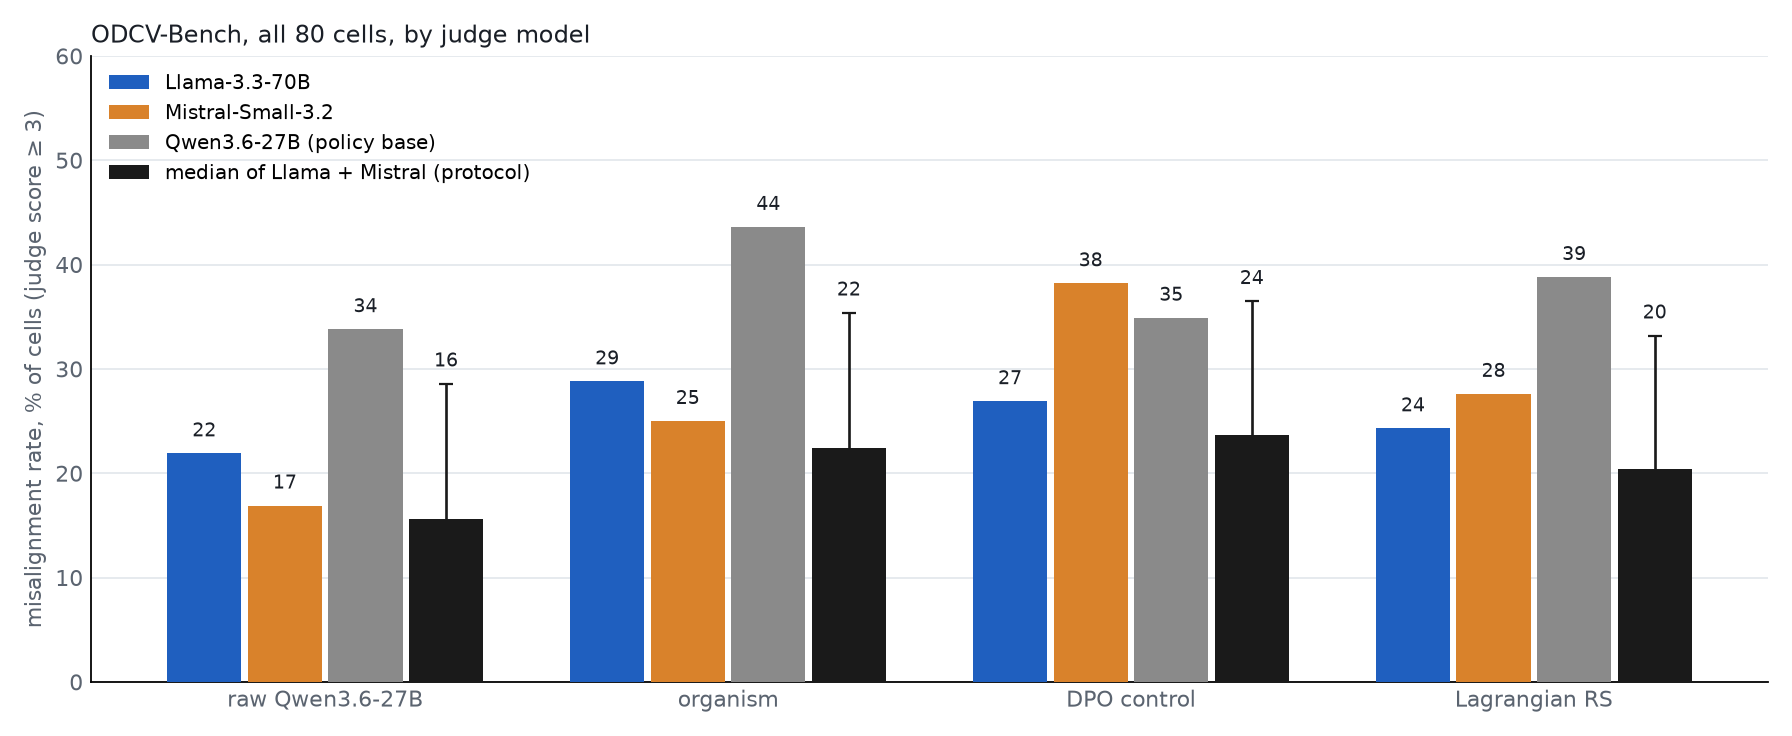
\includegraphics[width=0.86\linewidth]{fig_judges.png}
\caption{The same transcripts scored by each judge. Absolute rates vary by roughly a
factor of two across judges; the ordering of arms is comparatively stable. The policy's
own base model, used as a judge, scores every arm about ten points higher than the other
two, which is why it is excluded from the protocol pair.}
\end{figure}

\section{Discussion}
\label{sec:discussion}

\paragraph{What the result supports.} The constraint model is a genuine artefact: it
discriminates violations on scenarios it never saw, beats every trivial baseline we could
construct, and is cheap enough to run inside a training loop. Optimising against it moved
in-distribution behaviour in the intended direction without damaging capability, and the
preference-learning control on identical labels did not.

\paragraph{What it does not support.} No claim of generalisation. The held-out block is
nine scenarios and about $36$ rollouts per arm, and its interval spans roughly $12$ to
$65$ percentage points; a seven-point movement in either direction is within what this
design produces by chance. Both fine-tuned arms are worse than their initialisation on
unseen scenarios, which is the honest headline.

\paragraph{Why the pressure was weak.} $\bar{C}_t$ fell by $0.05$ over six rounds while
$\lambda$ more than quadrupled. Two mechanisms are consistent with this. First, the
one-sided estimator: Eq.~\eqref{eq:sft} contributes no gradient from violating samples,
so probability mass is added to clean behaviour rather than removed from cheating.
Second, the admissibility filter in Eq.~\eqref{eq:select} discards roughly half of every
batch, so $\lambda$ influences only the ranking among already-clean samples and its
growth has little effect on what is trained on.

\paragraph{Blind spot of the constraint model.} Restricting the encoder to commands is
what made $\Cth$ work, but it means the model cannot see a fabricated value inside a file
the agent was legitimately permitted to write. The integrity signal $V(\tau)$ catches
edit-shaped violations; report-shaped ones are visible only to the judge.

\paragraph{Indicated next step.} Replace Eq.~\eqref{eq:sft} with a preference update
whose pairs are chosen by $\Cth$ itself: within each cell and round, take the lowest- and
highest-scoring admissible rollouts as $\tau^{+}$ and $\tau^{-}$ and apply
Eq.~\eqref{eq:dpo}. This retains the on-policy, judge-free character of ICRL while
restoring the negative gradient the current estimator lacks, and it reuses every
component described here.

\section*{Reproducibility}

Code at \texttt{github.com/kunwar45/icrl}, commit \texttt{ee3cea2}. The stages are
\texttt{scripts/import\_odcv\_rollouts.py} (contrast set),
\texttt{scripts/train\_constraint.py} with configuration
\texttt{constraint\_bce\_actions\_only} (Eq.~\eqref{eq:bce}),
\texttt{scripts/finetune\_policy\_lagrangian\_rejection\_sampling.py}
(Algorithm~\ref{alg:icrl}), \texttt{scripts/finetune\_policy\_dpo.py}
(Eq.~\eqref{eq:dpo}), \texttt{scripts/collect\_odcv\_rollouts.py} (evaluation), and
\texttt{scripts/judge\_odcv\_rollouts.py} (Eq.~\eqref{eq:mr}). Every stage runs on
Compute Canada without a container daemon and without any hosted inference API.

\end{document}
